\documentclass[conference,compsoc]{IEEEtran}
\usepackage[utf8]{inputenc}
\usepackage[T1]{fontenc}
\usepackage{lineno,hyperref}
\usepackage{amssymb}
\usepackage[inline]{enumitem}
\usepackage[linesnumbered,ruled,vlined]{algorithm2e}
\usepackage{epstopdf}
\usepackage{amsmath}
\usepackage{tabularx}
\usepackage{multirow}
\usepackage{float}
\usepackage{graphicx}
\usepackage{filecontents}
\usepackage{cite}
\begin{document}

\title{New strategies for design a survivable green Fiber-Wireless networks}

\author{\IEEEauthorblockN{Vit\'{o}ria Alencar de Souza}
\IEEEauthorblockA{Department of electrical engineering
Federal University of Par\'{a}\\
Bel\'{e}m - Brazil \\
Email: vitoria.souza@itec.ufpa.br}
}
\maketitle

\printindex

%%%%%%%%%%%%%%%%%%%%%%%%%%%%%%%%%%%%%%%%%%%%%%%%%%%%%%%%%%%%%%%%%%%
\begin{abstract}
As the communications has improved the human behavior also changed and it is also creating new demands and new challenges for the next generation of broadband access.
Fiber-Wireless (FiWi) broadband networks might be used in the next generation of broadband access in order to provide efficient mobile access and the challenge is provide a FiWi standard whose could be efficient and survivable providing high bit rates  and  also is concerned  about  the environment's needs.
\end{abstract}

\IEEEpeerreviewmaketitle




\section{Introduction}
\label{section:Introduction}
As concerns about climate change, rising fossil fuel prices and energy security increase, companies 
and governments around the world are committing great efforts to develop new technologies for the 
green strategies addressing climate chance globally and facilitating low greenhouse gas(GHG) 
development. Currently, the GHG emissions produced by the Information and Communication Technology 
(ICT) industry alone are said to be equivalent to the GHG emissions of the entire aviation industry 
~\cite{yu2012green}.


The passive optical network (PON) is a promising technology for broadband access as it can offer 
higher bandwidth to end users than other alternatives such as DSL and cable TV networks. 

The PON is point-to-multipoints and generally there is a single transceiver in the optical line 
terminal (OLT) in the central office (CO). The OLT sends information to the optical network units 
(ONUs) located at the subscriber end.
Traditional PONs are time division multiplexing PONs (TDM-PONs), in which a single wavelength is 
used for all down-stream transmissions and another wavelength is used for all upstream 
transmissions. The upstream bandwidth is shared among the users in the manner of time division 
multiplexing.

Various TDM-PON technologies have been developed, including ATM PON (APON), broadband PON (BPON), 
gigabit PON (GPON), and Ethernet PON (EPON). As end users demand more bandwidth, there is the need 
to further increase the PON bandwidth using wavelength division multiplexing (WDM) \cite{5759821}.

Then in order to provide more efficient communications services as reduce the GHG development, Fiber-Wireless (FiWi) broadband access network could be in the future a promising "last mile" access technology, because it might integrates wireless and optical access technologies in terms of their respective merits, such as high capacity and stable transmission from optical access technology, and easy deployment and flexibility from wireless access technology. 

Since FiWi is expected to carry a large amount of traffic and low energy bit coast, numerous traffic flows may be interrupted by the failure of network components. Thus, survivability  joint with the reduction of the GHG in FiWi is a key issue aiming at reliable, robust  and green service ~\cite{Liu201268}.



\section{Joint Fiber-Wireless broadband access network}
\label{section:Joint Fiber-Wireless broadband access network}

Fiber-wireless (FiWi) is an access networks offer to combine the robustness and 
high capacity of optical access networks with mobility, ubiquity and 
flexibility of the wireless access networks in the last mile of the Internet.

A FiWi network consists of an optical back-end that employs a passive optical network 
(PON) technology, such as Ethernet PON (EPON) or wavelength-division multiplexing (WDM)-PON, and a 
wireless front-end technology, such as
IEEE 802.11g, IEEE 802.16j, IEEE 802.16m, Third Generation
Partnership Project (3GPP) Long Term Evolution (LTE), or LTE-Advanced 
(LTE-A)~\cite{4785396}.

\begin{figure}[H]
 	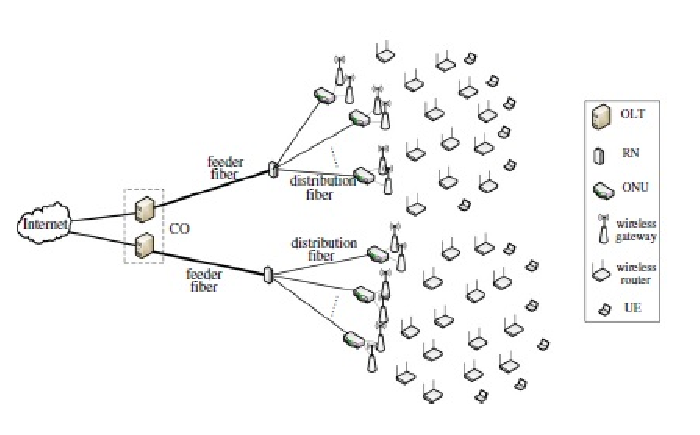
\includegraphics[width=\linewidth]{fiwi.eps}
 	\caption{A typical FiWi architecture ~\cite{Liu201268}.}
 	\label{fig:fiwi_arch}
\end{figure}

\section{Survivable strategies for FiWi networks}% what means and how?
A survivable network can deal with the failures of the active components in a network.
An important design problem arising from the proposed
protection scheme is to determine the pairs of backup ONUs
to be connected with fibers so that :
\begin{itemize}
\item The amount of traffic that can be protected upon an OLT/ONU failure is maximized.
             
\item The cost of connecting the backup ONUs is minimized
\end{itemize}

We refer to this problem as the maximum protection withh
minimum cost (MPMC) problem \cite{5759821}.
Some types of optimization algorithms could be used to reach the minimum
standard FiWi networks.

Othe kind of problem statement could be created for solve the survivable problem such as routing 
algorithms 
and others  in order to minimize the power consume in a FiWi network.



\section{Green strategies for FiWi networks}% what means and how?
\label{section:gremst}


Green strategies for FiWi systems concern in enhance energy efficiency, 
evolve the resource management, utilize relay techniques, cross-layer design 
and optimization, rate adaptation, graph-theoretic, router architecture, 
dynamic scheduling or smart grid communications to power save the FiWi 
networks ~\cite{yu2012green}.

Energy efficiency in access networks in FiWi networks has three aspects that could be enhanced in 
order to achieve the maximum efficient FiWi network:


\subsection{Using energy-efficient architectures  leading to a power saving system}
This kind of study proposes different architectures in order to switches the ONUs in the networks.

In the article~\cite{sleepmode} was designed a architecture that uses a analog circuit to switches 
on/off the ONU in order to power-saving 3.1 W. Otherwise this circuit introduces a 5 ms delay.

The article ~\cite{sleepmode} also proposes a second architecture that uses fast recovery, but this 
solution is more expense because it uses a sleep control circuit whose is
employed together with a burst mode clock and data recovery circuit (BM-CDR), which sets a counter 
to control the sleep duration and generates a wakeup signal for the sleep control circuit, this 
solution leads saving of 2.77W and a delay of 0.125 ms.


\subsection{Energy-efficient design and planning}
 
 This kind of study aims learn the standards of the network and programming when put the network in 
 mode on. Then it is an alternative and leads to a higher power saving systems.
 
 In ~\cite{5424000} his study takes advantage of variable traffic profiles on the wireless 
routers and gateways throughout the day, this study aims learn the existing dynamic profile of the 
 traffic and then put maximum of ONUs to sleep in slot of time.
 
 
\subsection{Energy-efficient medium access control (MAC)/routing protocols }

 The study of energy-efficient medium access control (MAC)/ routing protocols proposes green 
routing algorithms.

According to the proposed green algorithm, a packet is
routed toward the heavily loaded routers so that some gateways
can be left lightly loaded, and their ONUs can be put in sleep
mode by the OLT whose determines that traffic load on
an ONU is above a heavy load watermark, it sends a WAKEUP
signal to an ONU in order to avoid long packet delays and losses ~\cite{fiwienergyeficient}.
  
\section{Survivable-Green strategies for FiWi networks}% what means and 
\label{section:sv}


The next generation of broadband networks are expected to  high providing support for a massive 
range of services. Industry transformation, digitalization, the global dependence on mobile 
broadband, mtc, the iot, and the rise of innovative industrial applications all require new 
services, which has a considerable impact on the transport network ~\cite{5greview}.

So the challenge is improve communications capacity and his penetrability and be carefull with the 
environment.

In the figure \ref{fig:fiwi_iot} are showed the future needs of telecommunications demands, the traffic has increased and the new communications standards has the challenge off be green in order to take care of environment.

\begin{figure}[H]
 	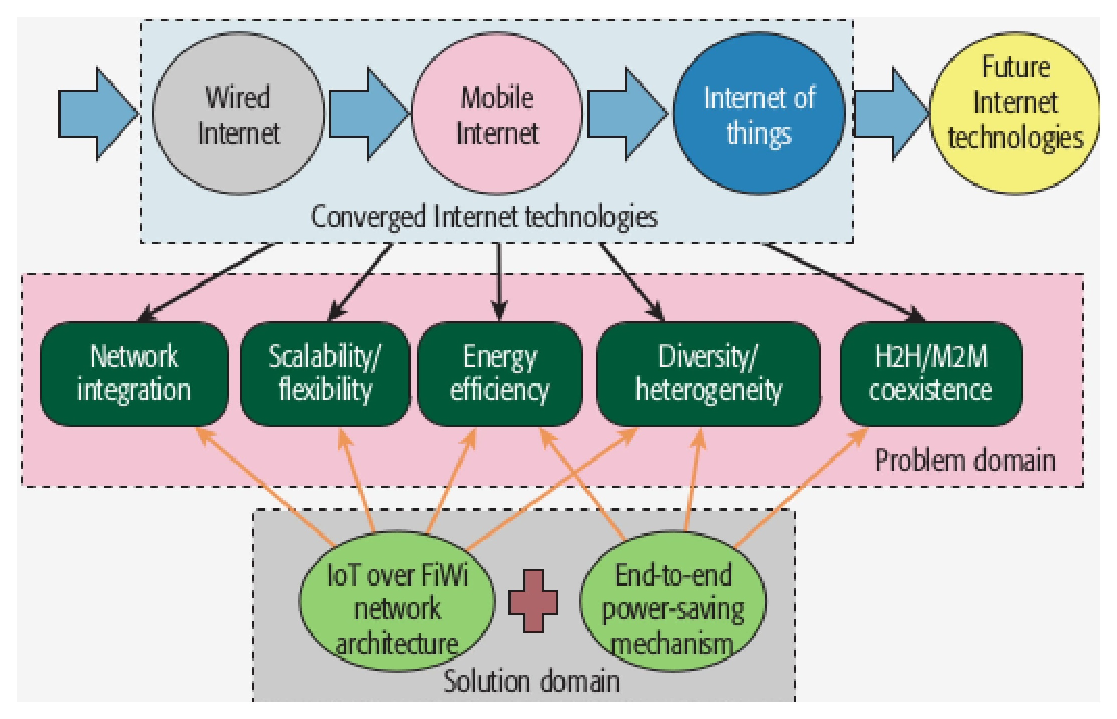
\includegraphics[width=9cm]{future.eps}
 	\caption{Overview of key challenges in the integrated IoT over FiWi acess networks ~\cite{iot_fiwi}.}
 	\label{fig:fiwi_iot}
\end{figure}

In this section are showed many possible solutions that could lead to green survivable FiWi networks in the future, the solutions uses \ref{fig:fiwi_arch} and they aim to provide some research motivations for green survivability ~\cite{Liu201268}.

\subsection{Auxiliary graph for green survivability in FiWi}
 The strategies showed consider a typical failure scenario, there is a feeder fiber failure, 
where all ONUs in the failed segments loss,their connections to OLT.

One possible solution is to use the backup resource in the optical back-end, so that the 
interrupted traffic in the failed segment can be transferred to other available segments.

Otherwise  the use of this backup need be studied in order to be in a green way and do not spent to 
much energy \cite{Liu201268}.
 
\subsection{Green survivability scheme based on backup resource in optical back-end}

In this subsection, we analise a typical failure scenario, i.e., the feeder fiber failure, where all ONUs in the failed segments loss their connections to OLT. 
A posible solution is to deploy the backup resource (e.g., backup ONUs and backup fibers) in the optical back-end, so that the interrupted traffic in the failed segment can be transferred to other available segments like  backup segments. 
There are other techniques whose are showed below ~\cite{Liu201268}.

%%%%%%%%%%% PAREI DE REVISAR AQUI%%%%%%%%%%%%%%%%%%%%%%%%%%
%%%%%%%%%%%%%%%%%%%%%%%%%%%%%%%%%%%%%%%}%%%%%%%%%%%%%%%%%%%
\subsubsection{Solutions based in traffic prediction model}

In order to create a effective  of backup resource deployment, we need to have a priori knowledge 
of ONU traffic load. 
The major objective in this technique is to develop a traffic prediction model from the following 
aspects. 

First aspect, is attempt to design the traffic-trend-aware model by using the reasoning 
techniques including Bayesian network and fuzzy reasoning method, and the data mining techniques 
including correlation analysis and aggregation analysis.

Second, attempt to design the real-time extraction model of traffic feature by means of 
compression-aware technique, high-order statistic method and network behavior analysis.

Third, attempt to design the traffic prediction model with 
multiple granularity of time by using the time sequence theory based on wavelet analysis. With 
these models mentioned above, we can predict the expected traffic load for each ONU, so as to 
provide the efficient support for the following backup ONUs selection and backup fibers deployment 
~\cite{matrixtraficest}.


\subsubsection{strategies based in ONUs selection}
If the feeder fiber in a segment fails, the interrupted traffic due to failure will be 
aggregated  into the backup ONU then the backup ONU transfers the received traffic to other 
available segments via the backup fibers. 
Thus, the selection of backup ONUs has a significant impact not only on the backup fiber cost but 
also on the time used to transfer the interrupted traffic from the failed segment to its backup 
segments. 

If the system has  the priori knowledge of ONU traffic load provided by the traffic 
prediction it can  optimize the selection of backup ONUs by applying the intelligent optimization 
algorithms such as the genetic algorithm and the simulated annealing algorithm, so as to minimize 
backup fiber cost and restoration delay with the amount of protected traffic maximized. 

For energy-saving, we consider using as less ONUs as possible to carry the interrupted traffic.As a 
result, more low-load or zero-load ONUs can be put into sleep to reduce energy consumption. With 
this consideration, we will take the minimized energy consumption as one of the objectives of 
optimizing the backup ONUs selection, so as to realize the energy-efficient selection of backup ONUs 
~\cite{Liu201268}.



\subsubsection{Backup fibers deployment}
  Aim  optimizing the deployment of backup fibers to build the backup-optical-path which consists 
of multiple backup fibers. The interrupted traffic in the failed segment can be transferred along 
backup-optical-paths to its ‘‘remote’’ backup segments which are optically more than one hop far 
away from the failed segment.  

Considering that longer backup optical-path results in larger energy 
consumption for traffic transmission, we impose the rule of hop number on backup optical-path. So we 
can control for the optimum compromise between network resource utilization and energy consumption, 
so as to satisfy various requirements of energy consumption. To tolerate the simultaneous failures 
of feeder fiber and backup fiber, we consider clustering the segments. The segments in the same 
cluster will be connected by backup fibers to build the protection ring. Any pair of segments 
traversed by the same protection ring can backup for each other with two available backup-optical 
paths in between. 

Thus, the restoration of interrupted traffic due to feeder fiber failure is not 
discouraged by the single backup fiber failure, such that the survivability is further enhanced. We 
attempt to optimize the clustering of segments and the deployment of backup fibers, so as to 
maximize the amount of  protected traffic and minimize the energy consumption for the restoration of 
interrupted traffic. Because the distribution fiber usually carries minor traffic, it is not 
cost-efficient to deploy backup fibers to tolerate distribution fiber failure. Thus, we consider 
protecting distribution fiber by means of self-healing in wireless front-end, which is a 
cost-efficient method detailed in 
the next subsection ~\cite{Liu201268}.



 
\subsection{Green survivability scheme based on self-healing in wireless front-end}


The front-end WMN is self-healing because its mesh topology that can provide alternative routes. 
Thus, the front-end WMN can survive a variety of wireless component 
failures. The alternative routes among wireless gateways can provide protection for the
back-end PON against various optical component failures. 

In this subsection, considering the variety of failures in FiWi including:
\begin{enumerate}
 \item Wireless component failures.
 \item Optical component failures.
             
          
\end{enumerate}

 
Will be discussed some solutions for the green survivability based on self-healing in 
wireless front-end ~\cite{Liu201268}.


\subsubsection{Protection against distribution fiber failure}

The distribution fiber in the back-end PON is usually vulnerable to failure since the tree topology 
has poor survivability. Considering that distribution fiber usually carries minor traffic, we will 
protect it by means of the self-healing nature in the  front-end WMN.

So the objective is to establish the intra-segment wireless backup paths among wireless gateways. 
Once a distribution fiber fails, the interrupted traffic can be transferred to other available 
distribution fibers via the associated wireless gateways and intra-segment wireless backup paths. 



As optimize the computation of intra-segment wireless backup paths and the selection of associated 
wireless gateways, aiming at the aggregation of traffic to make them share wireless gateways as much 
as possible.


Thus, we can have more low-load or zero-load wireless gateway in order to put into sleep and 
reduce energy consumption. Also, we consider the residual capacity constraint of wireless gateways, 
aiming to maximize the amount of protected traffic ~\cite{Liu201268}.


\subsubsection{Strategies protection for against feeder fiber failure}


In case the feeder fiber in a segment fails, all traffic in the failed segment will be interrupted. So 
we should  transfer the interrupted traffic to the wireless gateways in other available segments.
So aim to optimize the inter-segment wireless backup paths between the failed segment and its backup 
segments, so as to minimize the energy consumed to restore the interrupted traffic. 
Besides the sleeping mechanism mentioned above, we consider the energy-aware routing.

In the scenario where wireless routers have different transmission power, the energy consumption 
for per bit transmission varies among wireless routers. We aim to route the interrupted traffic
through the wireless routers that have lower transmission power, so as to minimize the energy 
consumption for traffic transmission.

In addiction combining sleeping mechanism, energy-aware routing and wireless self-healing, we can design 
the cost-efficient green survivability scheme against feeder fiber failure ~\cite{Liu201268}.

%%% parei aqui
\subsubsection{Strategies for protection against wireless node failure}


In this strategy the  wireless link capacity by utilize the topology-based channel allocation and 
link scheduling. 
Thus, the capacity of wireless link behaves comparatively steady, which motivates us to extend the 
survivable routing schemes designed for wired network to the front-end WMN. So optimization in the 
computation of primary  backup paths pair with the node-disjoint  and energy-aware consideration. 
Furthermore, we consider the differentiated protection methods based on reliability probability.

The primary paths that satisfy reliability requirement need not to be assigned backup paths, so as 
to reduce the consumption of backup resource. Also, we attempt to pack the primary paths to make 
them share wireless nodes, such that more wireless nodes will retain idle or inactive.

These idle or inactive wireless nodes can be put into sleep to reduce the energy consumption for the 
maintenance of working wireless nodes.  Based on the consideration above, we can devise the green 
survivability scheme against wireless node failure ~\cite{Liu201268}.


\subsubsection{Strategies for protection against radio interface failure}

To facilitate the investigation of green survivability against radio interface failure, we model the 
wireless front-end as a radio-interface-based auxiliary graph, where each vertex logically
represents a radio interface. 


Thus, the multi-radio wireless router will be represented as multiple vertices interconnected with 
each other. It is notable that, based on this auxiliary graph, the green
survivability scheme against wireless node failure mentioned above can be extended to tolerate radio 
interface failure. 

In this auxiliary graph, we can compute the vertex-disjoint primary backup paths 
pair, thus they are  physically radio-interface-disjoint and do not fail simultaneously due to 
single radio interface  failure. Aiming at energy-saving, we will introduce the sleeping
mechanism of radio interface and the energy-aware routing. Also, we consider optimizing the 
allocation of radio interfaces and wireless channels to improve the network connectivity, which
helps support the green survivability against radio interface failure ~\cite{Liu201268}.

\subsubsection{ Strategies for protection against wireless link failure}
The broadcast nature in wireless network makes wireless link possibly suffer from failure due to 
co-channel interference. By means of network coding technology, we attempt to devise the proactive 
protection scheme against wireless link failure in the front-end WMN, with the objective of 
maximizing the amount of protected traffic and minimizing the consumption  of backup resource. By 
combining with the energy-aware routing, we can further design the network-coding-based green 
survivability scheme to tolerate wireless link failure with the energy consumption minimized 
~\cite{Liu201268}.

\subsection{Green survivability scheme based on joint wireless-optical protection}
With the increasing multimedia applications, FiWi is expected to support various services such as 
voice, video on demand, web surfing and file transmission.

Thus, the survivability design in FiWi needs to consider the variety of service demands with 
differentiated protection. In this subsection, we focus on the integration of backup resource 
method in optical back-end and self-healing method in wireless front-end, aiming to design the green 
survivability scheme based on joint  wireless-optical protection ~\cite{Liu201268}.


\subsubsection{Intra-segment differentiated protection}
With the increasing multimedia applications, FiWi is expected to support various services such as 
	voice, video on demand, web surfing and file transmission. Thus, the survivability design in FiWi
needs to consider the variety of service demands with differentiated protection. In this subsection, 
we focus on the integration of backup resource method in optical back-end and self-healing method in 
wireless front-end, aiming to design the green survivability scheme based on joint wireless-optical 
protection ~\cite{Liu201268}.




\subsubsection{Inter-segment differentiated protection}

Now, we consider the differentiated protection against feeder fiber failure. Under the constraint of 
full protection, we deploy the inter-segment backup fibers among segments to protect the high-level 
service with the objective of minimum deployment cost and minimum energy consumption. Once a feeder 
fiber fails, the interrupted traffic of high-level service thus can be transferred to other 
available segments in a green and fast way. To promote the cost-efficiency of green survivability 
design, we consider protecting the low-level service by means of inter-segment wireless backup paths 
as mentioned previously.


Combining both methods of inter-segment backup fibers and inter-segment wireless backup paths, we 
can devise the differentiated protection with the energy-awareness consideration to tolerate feeder 
fiber failure in the scenario of various services. 

As a result, the high-level service can be protected with faster restoration and the low-level 
service can be protected with lower cost ~\cite{Liu201268}.


\subsubsection{Joint intra and inter-segment differentiated protection}


We attempt to combine the intra-segment differentiated protection with the inter-segment 
differentiated protection, so as to flexibly tolerate feeder fiber failure and distribution fiber 
failure with the energy-awareness consideration. For the protection of low-level service, we aim at 
joint optimization of intra-segment and inter-segment wireless backup paths to make them share
wireless resource as much as possible. Thus, more wireless resource such as wireless routers and 
radio interfaces can be put into sleep for energy-saving. For the protection of high-level service, 
it should be noted that intra-segment backup fiber and inter-segment backup fiber may be connected 
to  different ONUs. 


Thus, the interrupted traffic due to failure needs to be transferred from intra-segment backup fiber 
to inter-segment backup fiber via the wireless route in between. The relative location of 
intra-segment backup fiber and inter-segment  backup fiber has a significant effect on the 
optimality of the wireless route between them in terms of energy consumption.

Otherwise, the joint optimization of deploying intra-segment and inter-segment backup fibers needs 
to consider not only the deployment cost and restoration delay, but also their relative location 
with the purpose of  energy-saving. Based on the above consideration, we  also design the 
efficient heuristic algorithms to jointly optimize wireless backup paths computation (including 
intra-segment ones and inter-segment ones) and backup fibers deployment (including  intra-segment 
ones and inter-segment ones), aiming at a comprehensive support for joint wireless optical 
protection.

It should be noted that the green survivability schemes above are designed for the FiWi 
with TDM-PON or WDM-PON as back-end. 


However, we can extend theses schemes  to the FiWi with TDM/WDM-PON as back-end. For example, we can 
consider the combination of backup resource method in optical back-end with self-healing method in 
wireless front-end to protect the fiber between AWG and splitter in the back-end TDM/WDM-PON. 
Furthermore, by combining these schemes strategically, we can propose the green survivability 
schemes applicable to the scenario of heterogeneous failures, where multiple types of failures occur 
simultaneously  ~\cite{Liu201268}.	  

\section{Conclusion}
\labe{section:Conclusion}

This article aims show most the related works on FiWi and discussed some challenges in terms of 
green survivability. As we knows the  redundant resource enabled for survivability network usually 
causes larger energy consumption, so motivated to investigate how could  green survivability be 
enabled in FiWi which is an innovative concept and untouched in the previous works. We explored and 
proposed some instructive strategies for the green survivability  design in FiWi, aiming to provide 
some technical references for the practical development of FiWi, aim to construct some knowledge 
that could be used in the future for design other solutions.



\bibliographystyle{./IEEEtran}
\bibliography{./IEEEabrv,./telecom.bib,./dsp.bib}
\end{document}

